\newpage

\chapter{\textit{Firmware} ARON}

Kapitola je rozčleněna do několika sekcí,
které popisují hlavní funkce \textit{firmwaru} a jeho implementaci.
Každá sekce se zaměřuje na konkrétní oblasti, které jsou klíčové pro správný chod systému.
Struktura kapitol zhruba odpovídá hlavním třídám, jež se v \textit{\textit{firmwaru}} nacházejí.
Začínáme základním nastavením mikrokontroléru, které je nezbytné pro inicializaci celého systému,
pokračujeme přes popis komunikačních protokolů, implementaci regulátorů, metody řízení
až po hlavní smyčku a obslužná přerušení.


\section{Nastavení systému}
\label{section::System_settings}
Tato sekce popisuje základní nastavení mikrokontroléru a jeho inicializaci,
která je obsažena v souboru \texttt{system\_settings.hpp}.


\subsection{Konfigurace hodin}
Nejprve je nakonfigurován systém hodin.
Jako zdroj hodinového signálu GCLK2 je použit externí krystal s frekvencí \SI{20}{\mega\hertz}.
Tento signál je předdělen na \SI{1}{\mega\hertz} a použit jako GCLK1,
což usnadňuje další násobení ve dvou fázových závěsech (\texttt{DPLLx}).

\begin{figure}[htbp]
	\centering
	\includegraphics[width=0.9\textwidth]{kapitola4/figures/gclk_fig.png}
	\caption{Rozvod hodin \textit{GCLK} v mikrokontroléru \texttt{ATSAME51J20A} (převzato z \cite{ATSAME51J20A_ds}, s. 139)}
	\label{fig:Datasheet_gclk}
\end{figure}

\begin{itemize}
	\item Výstup z prvního fázového závěsu \texttt{DPLL1} poskytuje \SI{120}{\mega\hertz} jako GCLK0,
	      který slouží jako hlavní systémové hodiny a je využíván ve všech periferiích,
	      pokud není uvedeno jinak.
	\item Dělením frekvence GCLK0 vzniká GCLK3 s hodnotou \SI{30}{\mega\hertz} je využit pro taktování obou ADC.
	\item Výstup z druhého fázového závěsu \texttt{DPLL2} poskytuje GCLK4 s frekvencí \SI{200}{\mega\hertz} slouží pro taktování PWM čítače \texttt{TCC0}.
\end{itemize}

\subsection{Inicializace \texttt{ADC1}}
\label{section::system_settings}
AD převodník \texttt{ADC1} je zde inicializován a aktivován.
Periferie \texttt{ADCx} v tomto mikrokontroléru mají maximální doporčený taktovací kmitočet určený jako \SI{16}{\mega\hertz}.
Vzhledem k vytvořeným hodinám \texttt{GCLKx} byly vybrány hodiny \texttt{GCLK3} vydělené předděličkou dvěma na \SI{15}{\mega\hertz}.
Pro co možná nejpřesnější měření je jako referneční napětí je využito \SI{2,5}{\volt} z externí reference \textit{MCP1501T-25E},
viz \nameref{section::current_output}.
Převodník je nastaven jako \SI{12}{\bit} a po zahájení konverze automaticky průměruje \SI{64}{} po sobě jdoucích vzorků.
Teprve po ukončení průměrování nastavý flag \texttt{RESRDY}, který ohlašuje úspěšné ukončení konverze.
Dále je nastaveno, aby zahíjení konverze bylo možné spustit hardwarově,
jako reakci na libovolný flag přes \texttt{Event System}.
Převodníku \texttt{ADC1} je z \texttt{Event System} přiřazen kanál číslo \SI{14}.
Kdykoliv se objeví logická \SI{1} na tomto kanále, dojde automaticky k zahájení konverze.
Logickou jedničku jde v \texttt{Event System} možné nastavit softwarově,
na požadavek uživatele.

\begin{figure}[htbp]
	\centering
	\includegraphics[width=0.9\textwidth]{kapitola4/figures/evsys.png}
	\caption{Blok Event System v \texttt{ATSAME51J20A} (převzato z \cite{ATSAME51J20A_ds}, s. 783)}
	\label{fig:evsys}
\end{figure}

Vzhledem k plánovanému využití pro snímání z více pinů je zpracování výsledků konverze řízeno přerušením \texttt{ADC1}.
V rámci tohoto přerušení je vyhodnocen výsledek konverze na základě aktuálně nastavených vstupních pinů v registru \texttt{INPUTCTRL}.
Po dokončení konverze je vyvoláno přerušení, kde je zpracován výsledek z aktuálně snímaných pinů.
Po dokončení každé konverze je multiplexer automaticky přepnut na výchozí vstupní konektor \textbf{ADC1} na desce \emph{MoSeZ}.
Toto zajišťuje definovaný výchozí stav po každém zpracování výsledku.

\lstset{language=C++, basicstyle=\ttfamily\footnotesize, breaklines=true, captionpos=b}

\begin{lstlisting}[caption=Ukázka obsluhy ADC převodníku a multiplexeru vstupů, label=lst:adc_handler]
void adc1_1_handler() {
  switch (ADC1->INPUTCTRL.reg) {
    case (ADC_INPUTCTRL_MUXPOS_AIN0 | ADC_INPUTCTRL_MUXNEG_GND):
      // Měření teploty (AIN0)
      aron::adc1_temperature_read();
      ADC1->INPUTCTRL.reg = (ADC_INPUTCTRL_MUXPOS_AIN6 | ADC_INPUTCTRL_MUXNEG_GND); // Přepnutí na AIN6
      break;
    case (ADC_INPUTCTRL_MUXPOS_AIN6 | ADC_INPUTCTRL_MUXNEG_GND):
      // Měření pozice (AIN6)
      aron::Position_control::adc1_position_handler();
      break;
    case (ADC_INPUTCTRL_MUXPOS_AIN7 | ADC_INPUTCTRL_MUXNEG_GND):
      // Měření napětí na konektoru 2 (AIN7)
      float adc1_result_temp = (nd::utils::digital_to_analog_voltage(12, aron::Current_source::get_adc_vref(), ADC1->RESULT.reg));
      log().debug("{}", adc1_result_temp);
      ADC1->INPUTCTRL.reg = (ADC_INPUTCTRL_MUXPOS_AIN6 | ADC_INPUTCTRL_MUXNEG_GND); // Přepnutí zpět na AIN6
      break;
    default:
      ADC1->INPUTCTRL.reg = ADC_INPUTCTRL_MUXPOS_AIN6 | ADC_INPUTCTRL_MUXNEG_GND; // Výchozí stav: AIN6
      break;
  }
  ADC1->INTFLAG.bit.RESRDY = 1; // Vymazání příznaku přerušení
}
\end{lstlisting}

Kód ukazuje princip přepínání analogových vstupů pomocí registru \texttt{ADC1->INPUTCTRL}.
V každé větvi \texttt{switch} se nastavuje jiný vstup pro ADC převodník
(např. \texttt{AIN0} pro teplotní senzor, \texttt{AIN6} a \texttt{AIN7} pro další měření).
Po provedení měření se obvykle multiplexer přepne na další požadovaný vstup, nebo zpět na výchozí vstup.
Důležité je i mazání příznaku přerušení \texttt{RESRDY} po obsloužení požadavku.


\subsection{Ochrana proti přehřátí}

Pokud teplota překročí \SI{90}{\degreeCelsius},
výstup se automaticky vypne a současně se aktivuje červená \textit{LED} signalizující problém.
K opětovnému zapnutí nedojde pouhým poklesem teploty, výstup musí zapnout uživatel.


\subsection{Watchdog Timer}

Také zde dochází k inicializaci \textit{Watchdog Timer} \texttt{(WDT)}, což je periferie určená k monitorování správného běhu programu.
Jeho hlavním účelem je detekovat a umožnit zotavení se z chybových stavů, jako je například zablokování programu nebo nekontrolované vykonávání kódu.
Po aktivaci běží \texttt{WDT} nepřetržitě na základě předem definovaného časového limitu.
Pokud program neprovede vynulování (tzv. \textit{feeding}) \texttt{WDT} včas,
časovač vyvolá reset systému.
Kromě resetu lze využít také přerušení s předběžným varováním,
které signalizuje blížící se vypršení časovače
a v tomto přerušení podniknout kroky k obnovení chodu systému bez tvrdého restartu.
\texttt{WDT} je asynchronní a běží z nezávislého hodinového zdroje \texttt{OSCULP32K}, což znamená,
že funguje i v případě selhání hlavních systémových hodin.

\subsection{RAM ECC (Error Correction Code)}
RAM ECC zajišťuje vyšší spolehlivost systému detekcí a opravou paměťových chyb - automaticky opravuje jednobitové a detekuje dvoubitové chyby,
za cenu zabrání \SI{50}{\percent} celkové kapacity SRAM.
Aktivace probíhá zápisem do flash oblasti \texttt{USERROW} přes řadič \texttt{NVMCTRL},
přičemž před zápisem je nutné stránku kompletně vymazat.

\texttt{USERROW} obsahuje kromě ECC nastavení i kritické výrobní kalibrace.
Jakákoliv manipulace s touto oblastí vyžaduje extrémní opatrnost - nejprve je potřeba nahrát obsah do proměnné,
upravit pouze potřebné bity a poté provést zápis. Chybný zásah může \textit{MCU} zcela vyřadit z provozu.
\section{Interface}

Třída \texttt{Interface} zajišťuje inicializaci základních periferií systému, konkrétně \textit{LED} indikátorů,
tlačítka a komunikačního rozhraní \texttt{CAN} a \texttt{UART}.
Jejím cílem je připravit hardware pro správnou funkci a umožnit interakci s uživatelem i nadřazeným řídicím systémem.
Veškeré prvky jsou definovány jako statické atributy, což zajišťuje jejich snadnou dostupnost v celém programu.


\subsection{LED indikátory}

Zařízení disponuje třemi \textit{LED} indikátory,
které jsou pojmenovány jako \texttt{led\_green}, \texttt{led\_yellow} a \texttt{led\_red}.
Tyto diody slouží k vizuální signalizaci stavu systému.
Metoda \texttt{init\_led()} nastavuje všechny tři \textit{LED} jako výstupy a inicializuje je do výchozích stavů.
Ihned po spuštění systému se rozsvítí zelená a žlutá \textit{LED}, zatímco červená zůstává zhasnutá,
což umožňuje rychlou diagnostiku správného spuštění systému.
Během provozu se konfigurace rozsvícení diod mění dle aktuálního stavu zařízení.

Použití staticky definovaných instancí třídy \texttt{Gpio\_same5x} umožňuje přímou manipulaci s piny mikrokontroléru z libovolného místa v kódu.


\subsection{Tlačítko}

Tlačítko, pojmenované v kódu jako \texttt{button\_1},
je konfigurováno jako digitální vstup s aktivovaným vnitřním pull-up rezistorem,
což zajišťuje jeho stabilní stav při neuvedení do sepnuté polohy.
Pro detekci dlouhého stisku je využit časovač \texttt{TC2}, k
terý běží s hodinovým zdrojem \SI{1}{\mega\hertz} a využívá děličku frekvence \texttt{DIV64}.
Díky tomu lze přesně měřit dobu stisku tlačítka.
Časovač je nakonfigurován tak, aby vyvolal přerušení po přibližně 3 sekundách (\texttt{CC[0] = 46875}),
což umožňuje spolehlivou detekci dlouhého stisku a jeho odlišení od krátkého stisku.
Aktivace časovače probíhá v metodě \texttt{init\_button()},
kde se kromě konfigurace GPIO pinů nastavuje i přerušení pro \texttt{TC2}.
Přerušení je povoleno pomocí \texttt{NVIC\_EnableIRQ(TC2\_IRQn)}.
Obsluha tohoto přerušení je vyvolána po přetečení čítače,
což umožňuje systémové reakce na dlouhý stisk tlačítka.
Krátký stisk tlačítka je obsloužen v \texttt{main()} – pokud je tlačítko uvolněno před přetečením čítače \texttt{TCC2},
je stisk vyhodnocen jako krátký.

Krátký stisk tlačítka slouží k zapínání a vypnutí výstupu zařízení,
zatímco dlouhý stisk zajišťuje napřed vypnutí výstupu a poté restart celého systému.


\subsection{Třída \texttt{Logger}}

Třída \texttt{Logger} je implementována jako singleton, což znamená, že existuje pouze jedna instance loggeru v celém systému.
Tato instance je dostupná prostřednictvím metody \texttt{getLogger()}. Logger umožňuje nastavit jednotlivé úrovně záznamu
a poskytuje metody pro generování logovacích zpráv.
Každá zpráva je opatřena časovou značkou a výstupní formát je konstruován pomocí knihovny \texttt{fmt}.
Zprávy jsou poté předány metodě \texttt{log()}, která zajistí jejich odeslání do konkrétního výstupního zařízení.


\subsection{Třída \texttt{LoggerUart}}

Pro odesílání logovacích zpráv přes sériovou linku \texttt{UART} byla implementována odvozená třída \texttt{LoggerUart}.
Tato třída dědí z \texttt{Logger} a přepisuje metodu \texttt{log()}, která zajistí přenos zprávy prostřednictvím
ovladače \texttt{Usart\_blocking\_same5x}.


\subsection{Třída \texttt{CAN\_ATSAM\_C\_E}}

Třída slouží jako komplexní rozhraní pro práci s \textit{CAN} komunikací na mikrokontroléru \textit{ATSAM5X}.
Tento řadič sběrnice \textit{CAN} (Controller Area Network) je v systému realizován pomocí periferie \texttt{CAN1} a transceiveru \textit{TCAN334}.
Implementace třídy zahrnuje veškeré potřebné funkce – od inicializace a konfigurace periferie až po odesílání,
přijímání a filtrování zpráv, včetně zpracování chyb.

V konstruktoru třídy dochází k nastavení všech klíčových parametrů komunikace.
Konkrétně se jedná o konfiguraci pinů mikrokontroléru, aktivaci režimu \textit{CAN FD}, nastavení bitové rychlosti a konfiguraci filtrů zpráv.
Inicializace sběrnice \textit{CAN} probíhá v několika krocích.
Nejprve je nutné správně nakonfigurovat piny mikrokontroléru vyhrazené pro komunikaci a
povolit hodinový signál pro periferii. Následně je aktivován režim \textit{CAN FD}, který umožňuje vyšší přenosové rychlosti a
efektivnější komunikaci. Řadič \texttt{CAN1} je taktován generátorem \texttt{GCLK2} s frekvencí \SI{20}{\mega\hertz}.
Poté jsou nastaveny parametry časování, aby byla zajištěna optimální bitová rychlost.
Filtraci přijatých zpráv zajišťují standardní i rozšířené ID filtry,
které umožňují efektivně řídit, jaké zprávy budou zpracovány.

Pro příjem zpráv je využíván FIFO buffer, který po zpracování každou zprávu automaticky odstraňuje.
Odesílání zpráv funguje na principu vyrovnávací paměti (bufferu).
Zprávy se nejprve zapíší do bufferu a poté jsou odeslány po sběrnici.
Pokud není v bufferu dostatek volného místa, odeslání zprávy se neprovede, čímž se předchází zahlcení sběrnice.
Spolehlivost komunikace zajišťují implementované mechanismy pro detekci a zpracování chyb.
Třída dokáže rozpoznat chyby v přenosu, detekovat ztrátu zpráv a řešit další možné problémy,
které by mohly narušit správnou funkčnost \textit{CAN} sběrnice.


\subsection{Komunikační rozhraní}

Vytvořením instancí tříd \texttt{LoggerUart} a
\texttt{CAN\_ATSAM\_C\_E} unitř třidy \texttt{Interface} je inicializováno komunikační rozhraní systému.
Tyto tři výše jmenované třídy mi byly poskytnuty vedoucím práce, kterémuž tímto děkuji.
Pro účely ladění a diagnostiky je k dispozici sériový komunikační kanál \texttt{UART}.
Inicializace tohoto kanálu probíhá v metodě \texttt{init\_communication()},
kde je vytvořen objekt \texttt{LoggerUart}.
Tento objekt zajišťuje přenos dat prostřednictvím modulu \texttt{SERCOM4} s přenosovou rychlostí \SI{921 600}{\baud}.
Po úspěšné aktivaci \texttt{UART} kanálu je logger nastaven jako výchozí nástroj pro výpis zpráv.
Následně jsou do konzole odeslány úvodní inicializační zprávy.

Pro efektivní záznam událostí a ladění systému je implementována flexibilní struktura logování.
Tato struktura je založena na třídě \texttt{Logger},
která definuje několik úrovní závažnosti zpráv.
Mezi tyto úrovně patří \texttt{error} (chyba), \texttt{warn} (varování),
\texttt{info} (informace), \texttt{debug} (ladění), \texttt{CAN} a \texttt{CANopen}.
Díky této struktuře je možné snadno filtrovat a zaznamenávat pouze relevantní zprávy,
což usnadňuje proces ladění a diagnostiky.

Pro komunikaci desek mezi sebou je implementováno rozhraní \texttt{CAN}.
Hardwarovou vrstvu tvoří transceiver \texttt{TCAN334}, viz \nameref{section::CAN_Bus_Driver},
který je přes piny \texttt{PB13} a \texttt{PB12} propojen s řadičem sběrnice \texttt{CAN1}.

Metoda \texttt{init\_communication()} se stará o aktivaci transceiveru a inicializaci \texttt{CAN} řadiče.
Tento proces zahrnuje povolení napájení, nastavení režimu komunikace a konfiguraci odpovídajících GPIO pinů.
Tím je zajištěno, že zařízení je připraveno k přenosu a příjmu dat přes sběrnici \texttt{CAN}.

\subsection{Kompletní inicializace všech používaných interfaců}
Pro snadnou možnost inicializace periferií interface současně,
byla vytvořena metoda \texttt{init\_all()}.
Tato metoda postupně volá \texttt{init\_led()}, \texttt{init\_button()} a \texttt{init\_communication()},
čímž zajišťuje, že všechny nezbytné komponenty jsou správně nastaveny před zahájením hlavního běhu programu.


\section{Protokol komunikace po \texttt{CAN} a \texttt{UART}}
\label{section::comunication_protocol}

Sběrnice \textit{CAN} slouží k obecné komunikaci mezi zdroji.
Rozhraní \textit{UART} slouží jako jednoduchý kanál pro připojení jednoho zdroje \emph{MoSeZ} k PC.
Pokud je ovšem z PC adresován zdroj s jiným \textit{ID}, než je zdroj, který je připojen k PC,
dojde k automatickému přesměrování zprávy na sběrnici \textit{CAN}.

Přijatá zprává s validním \textit{ID} je předána metodě \texttt{aron::CommandHandler::message\_handler},
která zkontroluje správnost přijatých dat.
Pokud jsou přijatá data v pořádku,
je zpráva předána k vykonání, či předána k plnění sekvence.

Obě rozhraní dodržují formát zpráv ve tvaru stringu,
kde první je \textbf{Id}, pak \textbf{Příkaz} a nakonec \textbf{Data}.
Psáno bez oddělujících mezer tak, že:

\begin{center}
	\textbf{Id Příkaz Data}
\end{center}

kde:
\begin{enumerate}
	\item \textbf{Id} – identifikátor adresovaného zdroje,
	\item \textbf{Příkaz} – požadavek na adresovaný zdroj,
	\item \textbf{Data} – hodnoty předané zdroji.
\end{enumerate}

%===========================================================
\begin{table}[htbp]
	\centering
	\caption{Základní příkazy pro nastavení výstupu zdroje.
		*Pro zapnutí střídavého výstupu a řízení polohy je nutné nejprve nastavit tvar a frekvenci střídavého průběhu.}
	\begin{tabular} { | >{\centering\arraybackslash}m{3cm} | >{\centering\arraybackslash}m{3cm} | >{\raggedright\arraybackslash}m{8cm} | }
		\hline
		\textbf{Příkaz} & \textbf{Příklad} & \textbf{Popis}                                                                                                  \\
		\hline
		\texttt{I}      & \texttt{1I650}   & Požadovaná amplituda výstupního proudu. \newline Rozsah: \SI{-8000}{\milli\ampere} až \SI{8000}{\milli\ampere}. \\
		\hline
		\texttt{D}      & \texttt{1D1}     & Zapnutí/vypnutí DC výstupu. \newline 1 = zapnuto, 0 = vypnuto.                                                  \\
		\hline
		\texttt{A}      & \texttt{4A1}     & Zapnutí/vypnutí AC výstupu. \newline 1 = zapnuto, 0 = vypnuto.                                                  \\
		\hline
		\texttt{P}      & \texttt{1P1}     & Zapnutí/vypnutí řízení polohy voicecoilu. \newline 1 = zapnuto, 0 = vypnuto.                                    \\
		\hline
	\end{tabular}
	\label{tab:basic_commands}
\end{table}

%===========================================================\begin{table}[htpb]
%===========================================================
\begin{table}[htbp]
	\centering
	\caption{Příkazy pro nastavení průběhu a frekvence}
	\begin{tabular} { | >{\centering\arraybackslash}m{2.5cm} | >{\centering\arraybackslash}m{2.5cm} | >{\raggedright\arraybackslash}m{8.5cm} | }
		\hline
		\textbf{Příkaz} & \textbf{Příklad} & \textbf{Popis}                                                                                                                                       \\
		\hline
		\texttt{H}      & \texttt{1H50}    & Nastavení harmonického výstupu s~požadovanou frekvencí jako unsigned integer v~\SI{}{\hertz}. \newline Rozsah: \SI{1}{\hertz} až \SI{3000}{\hertz}.  \\
		\hline
		\texttt{T}      & \texttt{2T60}    & Nastavení trojúhelníkového výstupu frekvencí jako unsigned integer v~\SI{}{\hertz}. \newline Rozsah: \SI{1}{\hertz} až \SI{3000}{\hertz}.            \\
		\hline
		\texttt{S}      & \texttt{3S6000}  & Nastavení obdélníkového výstupu s~požadovanou frekvencí jako unsigned integer v~\SI{}{\hertz}. \newline Rozsah: \SI{1}{\hertz} až \SI{3000}{\hertz}. \\
		\hline
		\texttt{C}      & \texttt{2C75}    & Nastavení střídy obdélníkového výstupu v~procentech. \newline Rozsah: \SI{0}{\percent} až \SI{100}{\percent}.                                        \\
		\hline
		\texttt{RT}     & \texttt{3RT10}   & Nastavení doby náběhu obdélníkového signálu v~procentech periody. \newline Rozsah: \SI{0}{\percent} až \SI{50}{\percent}.                            \\
		\hline
		\texttt{F}      & \texttt{1F90}    & Nastavení fázového posunu výstupu ve stupních. \newline Rozsah: \SI{0}{\degree} až \SI{360}{\degree}.                                                \\
		\hline
		\texttt{O}      & \texttt{1O1000}  & Nastavení offsetu AC výstupu v~\SI{}{\milli\ampere}. \newline Rozsah: \SI{-6000}{\milli\ampere} až \SI{6000}{\milli\ampere}.                         \\
		\hline
	\end{tabular}
	\label{tab:waveform_commands}
\end{table}

%===========================================================
\begin{table}[htpb]
	\centering
	\caption{Příkazy použitelné pouze pro řízení polohy voicecoilu}
	\begin{tabular} { | >{\centering\arraybackslash}m{2.5cm} | >{\centering\arraybackslash}m{2.5cm} | >{\raggedright\arraybackslash}m{8.5cm} | }
		\hline
		\textbf{Příkaz} & \textbf{Příklad} & \textbf{Popis}                                                                                                                                                            \\
		\hline
		\texttt{R}      & \texttt{1R5000}  & Nastavení amplitudy polohy v~\SI{}{\milli\metre}. Hodnota je zadávána v tisícinách milimetru. \newline Součet offsetu a amplitudy musí být $\leq$ \SI{8.0}{\milli\metre}. \\
		\hline
		\texttt{V}      & \texttt{1V3500}  & Nastavení offsetu polohy v~\SI{}{\milli\metre}. Hodnota je zadávána v tisícinách milimetru. \newline Součet offsetu a amplitudy musí být $\leq$ \SI{8.0}{\milli\metre}.   \\
		\hline
	\end{tabular}
	\label{tab:position_commands}
\end{table}

%===========================================================
\begin{table}[htpb]
	\centering
	\caption{Systémové příkazy}
	\begin{tabular} { | >{\centering\arraybackslash}m{2.5cm} | >{\centering\arraybackslash}m{2.5cm} | >{\raggedright\arraybackslash}m{8.5cm} | }
		\hline
		\textbf{Příkaz} & \textbf{Příklad} & \textbf{Popis}                                                                                                               \\
		\hline
		\texttt{ID}     & \texttt{1ID2}    & Nastavení nového ID zdroje.                                                                                                  \\
		\hline
		\texttt{HB}     & \texttt{254HB1}  & Heartbeat pro potvrzení aktivity na sběrnici. \newline *ID zprávy HB = 254, data musí obsahovat ID zdroje, který HB odeslal. \\
		\hline
	\end{tabular}
	\label{tab:system_commands}
\end{table}
%===========================================================

\subsection{Sekvenční příkazy}

Pro rozsáhlejší možnost řízení výstupního signálu a jeho tvaru byla implementována funkcionalita sekvenčních příkazů,
která umožňuje uživateli definovat posloupnost změn parametrů výstupního signálu,
které se budou provádět v definovaném pořadí a v definovanou dobu.

Sekvenční příkazy se ukládají do pole struktur o maximální velikosti 100 příkazů.
Po splnění doby vykonávaného příkazu dojde k iteraci indexu ukazujícího na toto pole,
a tím se zahájí vykonávání další sekvence.
Tak se děje do doby vyčerpání všech příkazů uložených do tohoto pole struktur.

%===========================================================
\begin{table}[htpb]
	\centering
	\caption{Sekvenční příkazy}
	\begin{tabular} { | >{\centering\arraybackslash}m{2.5cm} | >{\centering\arraybackslash}m{2.5cm} | >{\raggedright\arraybackslash}m{8.5cm} | }
		\hline
		\textbf{Příkaz} & \textbf{Příklad} & \textbf{Popis}                                                          \\
		\hline
		\texttt{SP}     & \texttt{1SP1000} & Zahájení nové sekvence s~definicí doby trvání v počtu celých period.    \\
		\hline
		\texttt{SH}     & \texttt{1SH500}  & Zahájení nové sekvence s~definicí doby trvání v počtu půlperiod.        \\
		\hline
		\texttt{SW}     & \texttt{1SW200}  & Zahájení nové sekvence s~definicí doby vykonání v~\SI{}{\milli\second}. \\
		\hline
		\texttt{ST}     & \texttt{1ST0}    & Spuštění uložených sekvencí.                                            \\
		\hline
		\texttt{SC}     & \texttt{1SC0}    & Vymazání všech uložených sekvencí.                                      \\
		\hline
		\texttt{SF}     & \texttt{1SF0}    & Ukončení plnění nastavení aktuální sekvence.                            \\
		\hline
	\end{tabular}
	\label{tab:sequence_commands}
\end{table}

Systém zpracovává sekvenční příkazy tak, že nejprve přijímá zprávy z komunikačních rozhraní,
jako jsou \texttt{UART} nebo \texttt{CAN}.
Pokud se v metodě \texttt{aron::CommandHandler::comand\_exec()} detekuje příkaz pro zahájení nové sekvence (\texttt{SP}, \texttt{SH} nebo \texttt{SW}),
aktivuje se režim plnění sekvence. V tomto režimu jsou všechny následující příkazy interpretovány jako součást definice sekvence.
Každý příkaz je validován a jeho parametry jsou ukládány do interní struktury, která reprezentuje sekvenční příkaz.
Ukládání probíhá pro příkazy, které definují výstup, tedy \texttt{D}, \texttt{A}, \texttt{P}.
Jakmile je definice sekvence kompletní, interní struktura je předána do modulu pro správu sekvencí pomocí metody
\texttt{aron::CommandSequencer::add\_sequence\_command(const\ SequenceCommands \&sequence)}.
Po úspěšném přidání je režim plnění sekvence ukončen a interní struktura je resetována.

Pak je možné buď poslat nový příkaz, nový sekvenční příkaz, nebo spustit sekvenci již uložených příkazů pomocí příkazu \texttt{ST}.
Pokud je sekvence spuštěna, systém začne vykonávat jednotlivé příkazy v pořadí, v jakém byly uloženy.
Každý příkaz je vykonán po uplynutí definované doby, která byla uložena v sekvenčním příkazu.

\subsection{Validace příkazů}

Zařízení provádí validaci příkazů před jejich provedením.
Pokud příkaz nesplňuje požadovaná kritéria (např. hodnota mimo povolený rozsah),
je zamítnut a do logu je zaznamenána chybová zpráva.

Pro každý příkaz jsou definovány specifické omezení hodnot, které jsou uvedeny v~tabulkách výše.
Například:
\begin{itemize}
	\item Frekvence musí být v~rozsahu \SI{1}{\hertz} až \SI{3000}{\hertz}.
	\item Střída obdélníkového signálu musí být v~rozsahu \SI{0}{\percent} až \SI{100}{\percent}.
	\item Fázový posun musí být v~rozsahu \SI{0}{\degree} až \SI{360}{\degree}.
	\item Proudový OFFSET musí být v~rozsahu \SI{-6000}{\milli\ampere} až \SI{6000}{\milli\ampere}.
	\item Hodnota proudu musí být v~rozsahu \SI{-10000}{\milli\ampere} až \SI{10000}{\milli\ampere} (±\SI{10}{\ampere}).
\end{itemize}

%===========================================================
\subsection{Příklady použití kombinací příkazů}

Zde jsou uvedeny příklady použití kombinací příkazů pro běžné scénáře:

\textbf{Nastavení stejnosměrného proudu \SI{500}{\milli\ampere} na zdroji s ID 5}:
\begin{itemize}
	\item \texttt{"5I500\textbackslash n  5D1\textbackslash n"}
\end{itemize}

\textbf{Nastavení harmonického proudu \SI{1}{\ampere} s frekvencí \SI{50}{\hertz} na zdroji s ID 25}:
\begin{itemize}
	\item \texttt{"25I1000\textbackslash n  25H50\textbackslash n  25A1\textbackslash n"}
\end{itemize}

\textbf{Nastavení obdélníkového proudu \SI{2}{\ampere} s frekvencí \SI{100}{\hertz},
	střídou \SI{75}{\percent} a sklopením náběžných/doběžných \SI{20}{\percent} na zdroji s ID 250}:
\begin{itemize}
	\item \texttt{"250I2000\textbackslash n  250S100\textbackslash n  250C75\textbackslash n  250RT20\textbackslash n  250A1\textbackslash n"}
\end{itemize}

\textbf{Příklad uložení a spuštění sekvence 8 příkazů na zdroji s ID 1}:

\begin{itemize}
	\item \texttt{// 4 sekvence s časovým trváním 4 x 250 ms}
	\item \texttt{"1SW250\textbackslash n  1S100\textbackslash n  1I2000\textbackslash n  1A1\textbackslash n"}
	\item \texttt{"1SW250\textbackslash n  1S10\textbackslash n  1I1000\textbackslash n  1A1\textbackslash n"}
	\item \texttt{"1SW250\textbackslash n  1S50\textbackslash n  1I4000\textbackslash n  1A1\textbackslash n"}
	\item \texttt{"1SW250\textbackslash n  1H100\textbackslash n  1I1000\textbackslash n  1A1\textbackslash n"}
	\item \texttt{// 2 sekvence s trváním v celých periodách}
	\item \texttt{"1SP250\textbackslash n  1H125\textbackslash n  1I2000\textbackslash n  1A1\textbackslash n"}
	\item \texttt{"1SP250\textbackslash n  1S250\textbackslash n  1I4000\textbackslash n  1A1\textbackslash n"}
	\item \texttt{// 2 sekvence s trváním v celých periodách,}
	\item \texttt{// ale s výstupem aktivním jen v půlperiodě}
	\item \texttt{"1SH10\textbackslash n  1H5\textbackslash n  1I4000\textbackslash n  1A1\textbackslash n"}
	\item \texttt{"1SH2\textbackslash n  1S1\textbackslash n  1I1000\textbackslash n  1A1\textbackslash n"}
	\item \texttt{// Spuštění 8 příkazů uložené sekvence}
	\item \texttt{"1ST1\textbackslash n"}
\end{itemize}

\section{PID regulátor}

Pro řízení systému byla implementována třída \texttt{PID},
což je číslicová verze \textit{PID} regulátoru,
jehož výstup je počítán v metodě \texttt{OUT\_pid()}.
Tento regulátor byl navržen tak, aby umožňoval stabilní a přesné řízení požadované veličiny s možností omezení výstupu.
Následující sekce popisuje jednotlivé složky regulátoru a jejich implementaci.


\subsection{Omezení výstupu regulátoru}

Výstup regulátoru je omezen v rozsahu \(\langle u_{MIN}, u_{MAX} \rangle \) pomocí funkce \texttt{std::clamp()}.
Toto omezení zajišťuje, že regulátor nevygeneruje hodnoty,
které by byly mimo pracovní rozsah aktuátoru.
Hodnoty $u_{MIN}$ a $u_{MAX}$ jsou nastaveny při konstrukci třídy \texttt{PID}.


\subsection{Výpočet regulačního zásahu}

Výstup PID regulátoru je dán součtem tří složek: proporcionální, integrační a derivační.
Každá z těchto složek přispívá k celkovému regulačnímu zásahu a pomáhá dosáhnout požadované hodnoty regulované veličiny.

\begin{itemize}
	\item \textbf{Proporcionální složka (P)}
	      Proporcionální část regulátoru je dána součinem aktuální regulační odchylky a zesílení \(K_p \).
	      Tato složka reaguje okamžitě na změny v řízeném systému, ale při trvalé odchylce nemusí být schopna dosáhnout nulové chyby.
	      V implementaci je vypočtena jako:
	      \begin{equation}
		      P = K_p \cdot e(k)
	      \end{equation}

	\item \textbf{Integrační složka (I)}
	      Integrační složka zajišťuje eliminaci ustálené regulační odchylky tím, že akumuluje součet předchozích chyb.
	      Implementována je numericky pomocí metody obdélníkového pravidla s průměrnou hodnotou dvou po sobě jdoucích chyb.
	      Výpočet probíhá dle rovnice:
	      \begin{equation}
		      I(k) = I(k-1) + 0.5 \cdot K_i \cdot T_s \cdot (e(k) + e(k-1))
	      \end{equation}
	      kde \(T_s \) je vzorkovací perioda.
	      Pro zamezení nasycení integrátoru je jeho hodnota omezena pomocí funkce \texttt{std::clamp()} v mezích \(\langle 0.2 \cdot u_{MIN}, 0.2 \cdot u_{MAX} \rangle \).

	\item \textbf{Derivační složka (D)}
	      Derivační složka slouží k predikci budoucího chování systému na základě změny regulační odchylky.
	      K jejímu výpočtu se využívá diference dvou po sobě jdoucích chyb, čímž se přibližně počítá její derivace:
	      \begin{equation}
		      D = K_d \cdot \frac{e(k) - e(k-1)}{T_s}
	      \end{equation}
	      Derivační složka je následně filtrována digitálním filtrem prvního řádu s koeficientem \(\beta \),
	      aby se zamezilo amplifikaci šumu:
	      \begin{equation}
		      D_f = (1 - \beta) \cdot D_f + \beta \cdot D
	      \end{equation}
\end{itemize}

\textbf{Celkový regulační zásah ($PID_{OUT}$)} je dán součtem všech tří složek:
\begin{equation}
	PID_{OUT} = P + I(k) + D_f
\end{equation}


\subsection{Experimentální ladění regulátoru}

Jsou vytvořeny dvě instance \texttt{PID} regulátoru, jedna pro regulaci proudu a
druhý pro regulaci polohy.
Koeficienty \(K_p, K_i, K_d \) byly stanoveny experimentálně na základě odezvy systému na skokovou změnu požadované hodnoty.
Cílem bylo najít takové hodnoty, které zajistí dostatečně rychlou odezvu bez většího překmitu a současně stabilní regulaci v ustáleném stavu.
K ověření správné funkce regulátoru byly výstupy sledovány pomocí osciloskopu.
Implementovaný regulátor se osvědčil při řízení proudu a polohy v aktuátoru.


\section{Regulace proudu}
\label{section::current_output}

Tato sekce se zabývá regulací proudu,
zahrnující inicializaci a konfiguraci převodníku \texttt{ADC0} pro měření proudu,
použití čítače \texttt{TCC0} k generování \textit{PWM} signálu a
řízení \textit{H-můstku} s ohledem na minimalizaci ztrát a ochranu tranzistorů.
Popisuje strategii řízení \textit{H-můstku} v závislosti na regulační odchylce a
využití \textit{PID} regulátoru pro přesnou regulaci proudu.
Dále vysvětluje použití atomických proměnných k bezpečnému sdílení požadavku na proud mezi hlavním programem a přerušením,
čímž se zajišťuje spolehlivost a konzistence dat při regulaci.

\subsection{Inicializace převodníku \texttt{ADC0}}

Inicializace probíhá ve funkci \texttt{Current\_source::init()}.
Nejprve je povolen hodinový signál pro \texttt{ADC0} jako \SI{30}{\mega\hertz} \texttt{GCLK3}
vydělených předděličkou v \texttt{ADC0} na \SI{15}{\mega\hertz}.
Takový kmitočet byl zvolen ze stejných důvodů jako pro \texttt{ADC1} v \nameref{section::system_settings}.
Poté je nakonfigurován pin \texttt{PA06},
který vede k externímu difereniálnímu zesilovači \textit{INA241B1}.
Tento zesilovač snímá úbytek napětí na snímacím odporu zapojeném do série se zátěží a
tím poskytuje informaci o aktuálním proudu pro zpětnou vazbu regulátoru.
Následně je nakonfigurován \texttt{ADC0}, včetně prescaleru,
externí reference \textit{MCP1501T-25E}, kalibrace a hardwarového průměrování na 2 vzorky.
Dále je povoleno přerušení po dokončení převodu a nastaveno spouštění převodu událostí.

\begin{figure}[htpb]
	\centering
	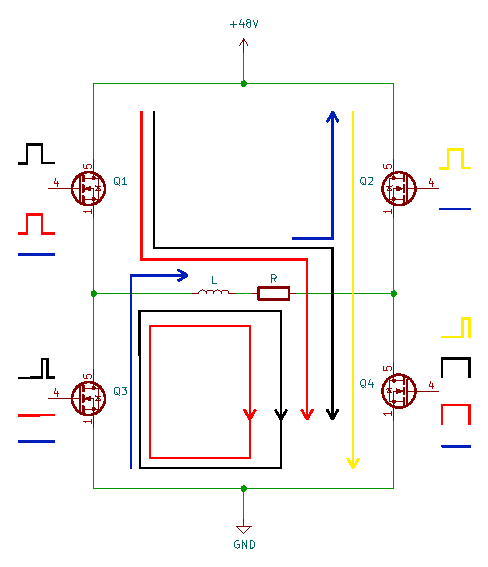
\includegraphics[width=0.7\linewidth]{kapitola4/figures/hbridge_driving.eps}
	\caption{Vše uvažováno pro kladný směr proudu.  Vyznačeného \textbf{černě} pro spínání tranzistorů pro regulační odchylku menší než \SI{5}{\percent} požadovaného proudu,
		\textbf{modře} pro naakumulovanou energii v indukčnosti a vypnuté tranzistory,
		\textbf{žlutě} pro nechtěné současné sepnutí tranzistorů jedné větve}
	\label{fig:mosfet_driving}
\end{figure}


\subsection{Popis a inicializace čítače \texttt{TCC0}}

Pro generování \textit{PWM} signálu pro řízení driverů \textit{MP1917} je čítač \texttt{TCCx} ideální volbou,
neboť některé jeho funkce usnadňují řízení H-můstků.
Funkce \texttt{Non-Recoverable Fault (NRF)} zajišťuje předem definované chování tranzistorů v případě detekce \texttt{NRF},
což je jinými slovy událost \texttt{EVENT\_1} na programátorem definovaném kanálu
(v našem případě nastaveno na kanálu \SI{2}) periferie \texttt{Event\ System}).

Při detekci \texttt{NRF} jsou rozepnuty horní tranzistory  (\textit{Q1} a \textit{Q2} v obr. \ref{fig:mosfet_driving}) a
sepnuty dolní tranzistory \textit{H-můstku} (\textit{Q3} a \textit{Q4} v obr. \ref{fig:mosfet_driving}),
čímž se vytvoří cesta pro vybití energie z indukční zátěže.
Takové chování ilustruje černá smyčka přes tranzistory \textit{Q3} a \textit{Q4} v obr. \ref{fig:mosfet_driving}.


V případě pouhého vypnutí všech tranzistorů si potenciálně naakumolovaná energie v induknčnosti \textit{L}
otevře cestu přes zpětné diody tranzistorů, jak pro kladný směr proudu naznačuje modrá smyčka v obr. \ref{fig:mosfet_driving}
přes zpětné diody tranzistorů \textit{Q2} a \textit{Q3}.
Tímto způsobem se indukčnost \textit{L} sice vybije,
ale hrozí vznik nežádoucího napěťového přepětí ve stejnosměrném meziobvodu.
Proto je jakákoliv deaktivace výstupu realizována generováním \texttt{NRF},
respektive generováním \texttt{Event} na kanálu \SI{2}{},
což zajišťuje bezpečné vybití energie z indukčnosti \textit{L}
a pozastavení čítače \texttt{TCC0} do doby deaktivace \texttt{NRF}.

Další užitečnou funkcí je automatické vkládání \textit{dead-time} mezi spínáním \textit{high-side}
a \textit{low-side} tranzistorů v jedné větvi.
Otevřený tranzistor se totiž zavírá s určitou setrvačností po změně řídícího signálu \textit{gatu} na \SI{0}{\volt},
díky čemuž může dojít ke zkratu napájecího napájení v oné větvi, viz fialově vyznačený proud v obr. \ref{fig:mosfet_driving}).
Vložením vhodně dlouhé doby, kdy se čeká než dojde k sepnutí opačného tranzistoru jedné větve, takzvaný \textit{dead-time},
se předchází zbytečným ztrátám či dokonce destrukci tranzistorů.

Při inicializaci je nejdříve v čítači \texttt{TCC0} povolen hodinový signál a nakonfigurovány piny \texttt{PA20} až \texttt{PA23}.
Registr \texttt{Output Matrix} je nastaven tak,
že \texttt{PA20} a \texttt{PA21} řídí \textit{low-side} tranzistory \textit{Q3} a \textit{Q4},
a \texttt{PA22} a \texttt{PA23} řídí \textit{high-side} tranzistory \textit{Q1} a \textit{Q2} (viz obr. \ref{fig:mosfet_driving}).
Každému výstupnímu pinu odpovídá \texttt{Capture Compare} registr se stejným indexem \texttt{PA2x}:

\begin{table}[htpb]
	\centering
	\caption{Přiřazení CCx registrů k pinům PA20 až PA23}
	\label{table::OTMX_CC_to_PA}
	\begin{tabular}{ll}
		CC0 & PA20 \\
		CC1 & PA21 \\
		CC2 & PA22 \\
		CC3 & PA23 \\
	\end{tabular}
\end{table}

Perioda čítače je nastavena na \SI{2000}{}, což při vstupním kmitočtu \SI{200}{\mega\hertz},
generuje \textit{PWM} s kmitočtem \SI{100}{\kilo\hertz}.
Vložený \textit{dead-time} mezi spínání high a low side tranzistorů jedné větve je \SI{10}{\nano\second},
Je povoleno generování přerušení při přetečení, \texttt{NRF} a jeho registry,
které defunují stavy jednotlivých výstupů při detekci \texttt{NRF}.


\subsection{Řízení H můstku}

Regulační smyčka obsahuje \textit{PID} regulátor,
jehož konstanty byly experimentálně naladěny na základě odezvy systému na obdélníkový požadavek změny proudu a
jeho výsledného průběhu na zátěži. Jako zátěž byla použita indukčnost o velikosti \SI{250}{\micro\henry},
což odpovídá minimální očekáváné hodnotě v budoucnu používaných aktuátorů a akčních členů.
Samotná \textit{DPS} zdroje neobsahuje žádnou filtrační indukčnost,
neboť předpokládané zátěže jsou vždy induktivního charakteru.

\begin{figure}[htpb]
	\centering
	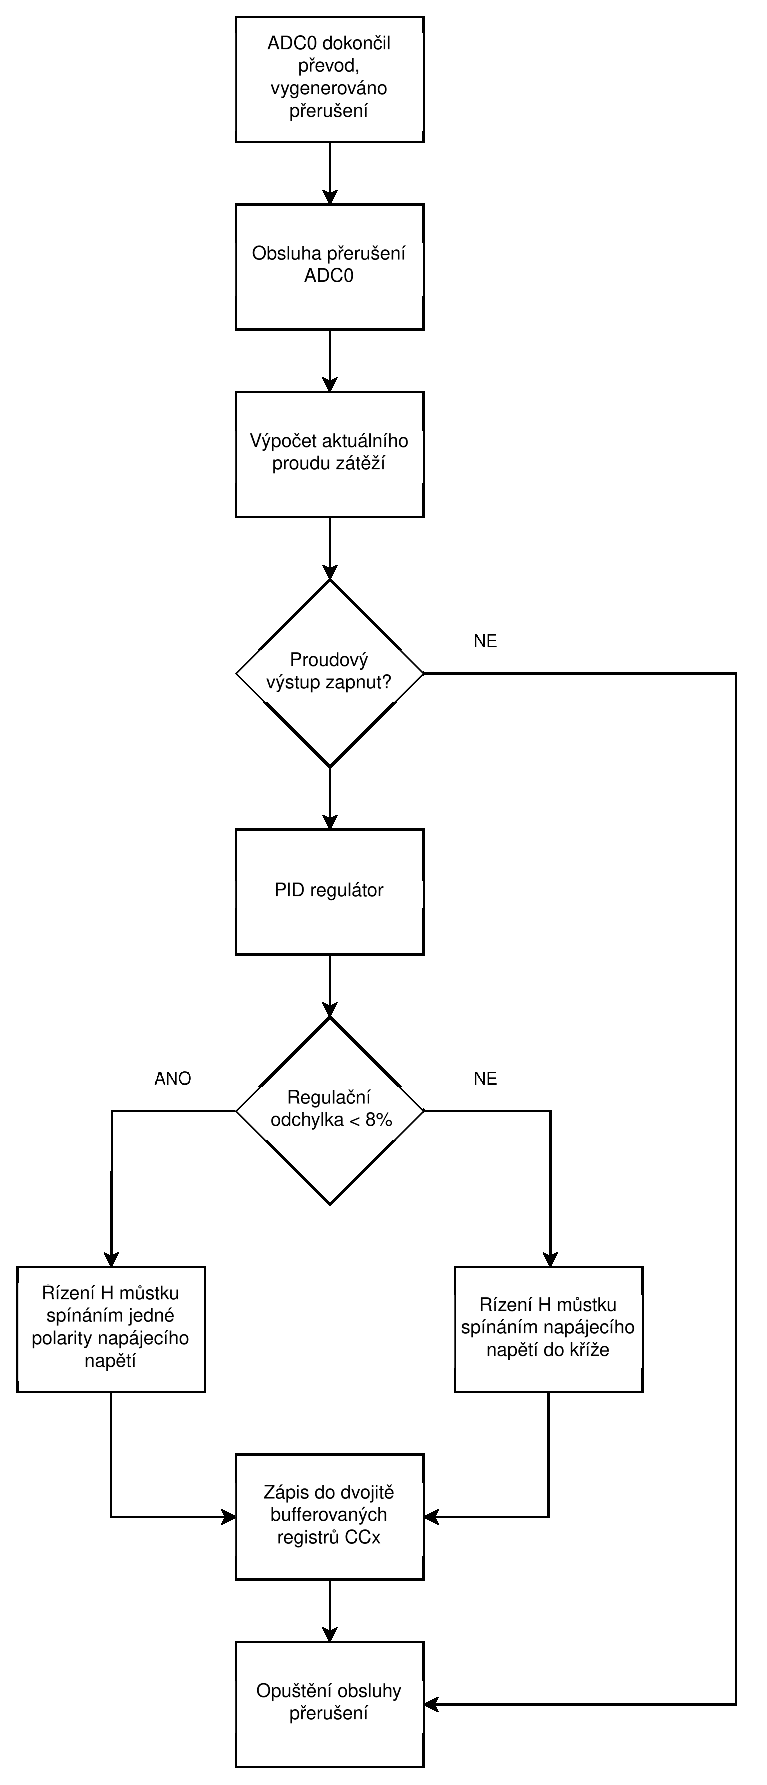
\includegraphics[width=0.6\linewidth]{kapitola4/figures/flowchart_regulator_current.eps}
	\caption{Vývojový diagram proudové regulace}
	\label{fig::flowchart_regulator_curret}
\end{figure}

Vývojový diagram regulace proudu je vidět na obrázku \ref{fig::flowchart_regulator_curret}.
Spuštění regulační smyčky je vázáno na dokončení převodu \texttt{ADC0} a podmíněno povolením proudového výstupu.
Zahájení převodu \texttt{ADC0} je iniciováno přetečením čítače \texttt{TCC0}.
Převodník \texttt{ADC0} je určen výhradně pro měření napětí na proudovém senzoru \textit{INA241B1}.
Po dokončení převodu je vyvoláno přerušení, ve kterém je vypočítána aktuální hodnota proudu na základě změřeného napětí a
převodní konstanty senzoru. Regulační odchylka, definovaná jako rozdíl mezi požadovanou a naměřenou hodnotou proudu,
je následně předána PID regulátoru, který vypočítá nové hodnoty \texttt{CCx} registru čítače \textit{TCC0}.

V kódu je nejdříve vypočítána prahová hodnota regulační odchylky \texttt{error\_th} jako \SI{5}{\percent}
z požadovaného proudu \texttt{current\_request}.
Tato hodnota je následně omezena funkcí \texttt{std::clamp} tak,
aby nebyla menší než \SI{300}{\milli\ampere} a větší než \SI{1000}{\milli\ampere}.
Funkce \texttt{std::clamp} tedy zajišťuje,
že prahová hodnota bude vždy v rozmezí od \SI{300}{\milli\ampere} do \SI{1000}{\milli\ampere},
i když by \SI{5}{\percent} z požadovaného proudu bylo mimo tento rozsah.

Tato prahová hodnota se poté porovnává s aktuální regulační odchylkou \texttt{error\_current}.
Pokud je absolutní hodnota regulační odchylky větší než \texttt{error\_th},
tedy pokud se nachází mimo interval $\langle -\texttt{error\_th}; \texttt{error\_th} \rangle$,
H-můstek řídí proud spínáním tranzistorů do kříže.
Tím je na zátěž přivedena buď kladná, nebo záporná polarita napájecího napětí,
což umožňuje rychlou změnu proudu a velký akční zásah.

Pokud však regulační odchylka zůstává v intervalu $\langle -\texttt{error\_th}; \texttt{error\_th} \rangle$,
strategie řízení se mění:
\begin{itemize}
	\item Trvale je sepnut jeden z \textit{low-side} tranzistorů (podle směru proudu).
	\item Střídavě se spíná \textit{high-side} a \textit{low-side} tranzsitor větve opačné, viz černý průběh na \oref{fig:mosfet_driving}
\end{itemize}

Tento způsob řízení snižuje strmost změn napětí na zátěži,
čímž se snižuje zvlnění proudu a omezuje rušení, zejména u zátěží s malou indukčností.
Zkratování zátěže v opačných cyklech je nezbytné,
aby indukční zátěž mohla k uzavření obvodu využít otevřených tranzistorů namísto jejich zpětných diod,
viz červený průběh na obrázku \ref{fig:mosfet_driving}.
To by způsobovalo zbytečné ztráty,
protože zpětné diody mají větší úbytek napětí než otevřené tranzistory.

Při návrhu byla zohledněna požadovaná rychlost regulační smyčky,
aby bylo možné vypočítat novou hodnotu střídy \textit{PWM} v každé periodě čítače \texttt{TCC0},
což bylo ověřeno experimentálně.
Testování probíhalo tak,
že na začátku regulační smyčky byla aktivována jedna z \textit{LED} a při jejím dokončení byla \textit{LED} opět vypnuta.
Na osciloskopu byl sledován průběh napětí na \textit{LED} a řídicí signály \textit{H-můstku},
přičemž přetečení čítače \texttt{TCC0} bylo na osciloskopu jasně patrné, stejně tak jako i sepnutí a vypnutí signálů LED
Tyto experimenty potvrdily schopnost výpočtu nového regulačního zásahu v každém vzorkovacím okamžiku \texttt{ADC0}.


\subsection{Využití proměnných \texttt{std::atomic}}

Požadovaná hodnota proudu je stanovena uživatelem a uložena
jako amplituda v proměnné \texttt{current\_request}.
Pro stejnosměrný výstup je tato hodnota přímo použita jako referenční proud pro regulaci.
U střídavého výstupu dochází k přenásobování této proměné v metodě přímé digitální syntézy (\textit{DDS}).

V režimu regulace polohy voicecoilu slouží výstup z regulátoru polohy jako požadavek na proud,
tedy opět proměná \texttt{current\_request}, ukládající požadavek na proud.
Proměná je tedy sdílena mezi hlavním programem (zpracování zprávy, viz \nameref{section::mcu_main_run}),
regulátorem proudu (přerušení \texttt{ADC0}), regulátorem polohy (přerušení \texttt{ADC1}, viz \nameref{section::position_regulator})
a \textit{DDS} (přerušení \texttt{TC0}, viz \nameref{section::dds_implementation}).
Výše jmenované úlohy jsou spouštěné nesekvenčně,
všechny zmíněné periferie používají různé kmitočty a
navíc ve všech jmenovaných přerušeních dochází k možnému zápisu do proměné \texttt{current\_request}.
Z tohoto důvodu je pro \texttt{current\_request} použit typ \texttt{std::atomic<float>}.

Standardní proměnné v \textit{C++} nejsou ve výchozím nastavení \textit{thread-safe}, což znamená,
že pokud k nim přistupuje více vláken nebo přerušení současně, může dojít k problémům,
jako je \textit{race condition} nebo \textit{data corruption}.
\texttt{std::atomic} je třída v \textit{C++}, která poskytuje atomické operace.
Atomické operace jsou nedělitelné, což znamená, že se buď provedou celé, nebo vůbec.
Díky tomu je zajištěno, že i když k proměnné přistupuje více vláken nebo přerušení současně,
nedojde k nekonzistenci dat.
Použití atomických proměnných je důležité zejména v těchto situacích:

\begin{itemize}
	\item \textbf{Sdílení dat mezi přerušením a hlavním programem:} Přerušení může zapisovat do proměnné, kterou hlavní program čte. Bez atomických operací by mohlo dojít k tomu, že hlavní program čte nekompletní nebo nekonzistentní data.
	\item \textbf{Sdílení dat mezi více vlákny:} Pokud více vláken přistupuje ke stejné proměnné, atomické operace zajistí, že nedojde k \textit{race condition}.
	\item \textbf{Synchronizace:} Atomické proměnné mohou být použity pro synchronizaci mezi vlákny nebo přerušením a hlavním programem.
\end{itemize}


\section{Regulace polohy}
\label{section::position_regulator}

Pro určení polohy slouží převodník \texttt{ADC1},
který je ihned po startu dedikován k měření teploty jednou za \SI{10}{\second},
viz \nameref{section::System_settings}.
Nicméně v obsluze jeho přerušení bylo dopředu počítano s multiplexem různých vstupů.
Převodník \texttt{ADC1} byl zvolen pro multiplex,
neboť druhý dostupný převodník \texttt{ADC0} využívaný pro měření výstupního proudu je využit na hranici své datové prostupnosti.

Převodník \texttt{ADC1} je nakonfigurován pro měření napětí z Hallovy sondy připojené ke třípinovému konektoru.
Tato sonda poskytuje regulátoru polohy informaci o aktuální poloze jádra lineárního aktuátoru.
Zahájení převodu je řízeno přetečením čítače \texttt{TCC0}, který zároveň generuje \textit{PWM} signál pro řízení \textit{H-můstku}.
Událost přetečení čítače je zpracována pomocí modulu \texttt{Event System},
který umožňuje zahájení převodu bez zásahu hlavního procesoru.
Převodník \texttt{ADC1} reaguje na událost \texttt{EVENT\_0} generovanou čítačem \texttt{TCC0},
pouze pokud je povolena regulace polohy, v opačném případě slouží pouze pro měření teploty.

Po ukončení převodu generuje \texttt{ADC1} přerušení, v jehož obsluze je volán regulační algoritmus pro řízení polohy.
Tento proces se opakuje s periodou přibližně $\approx$~\SI{220}{\micro\second},
která je výrazně delší než samotná perioda přetečení čítače \texttt{TCC0}, a tudíž i generace \textit{PWM}.
Eventy generované čítačem \texttt{TCC0} během aktivního převodu \texttt{ADC1} jsou jednoduše ignorovány.

Výpočet periody převodu AD převodníku je dán vztahem:

\begin{equation}
	T_{\text{ADC}} = \frac{f_{\text{ADC\_CLK}}}{(N_{\text{RES}} + 1) \cdot N_{\text{SAMPLES}}}
	\label{eq:T_ADC1}
\end{equation}

kde:

\begin{itemize}
	\item $f_{\text{ADC\_CLK}}$ – hodinová frekvence převodníku (\SI{15}{\mega\hertz}),
	\item $N_{\text{RES}}$ – bitová hloubka převodu (zde \SI{12}{\bit}),
	\item $N_{\text{SAMPLES}}$ – počet vzorků pro hardwarové průměrování (v tomto případě \num{256}).
\end{itemize}

Dosazením těchto hodnot do rovnice~\eqref{eq:T_ADC1} získáme:

\begin{equation}
	T_{\text{ADC}} = \frac{15 \times 10^{6}}{(12 + 1) \cdot 256} \approx \SI{220}{\micro\second}
	\label{eq:T_ADC1_evaluated}
\end{equation}

Převodník \texttt{ADC1} je navíc periodicky využíván pro měření teploty desky.
Tato měření však probíhají pouze jednou za \SI{10}{\second},
a jejich vliv na vzorkovací frekvenci Hallovy sondy je z praktického hlediska zanedbatelný.


\begin{figure}[htpb]
	\centering
	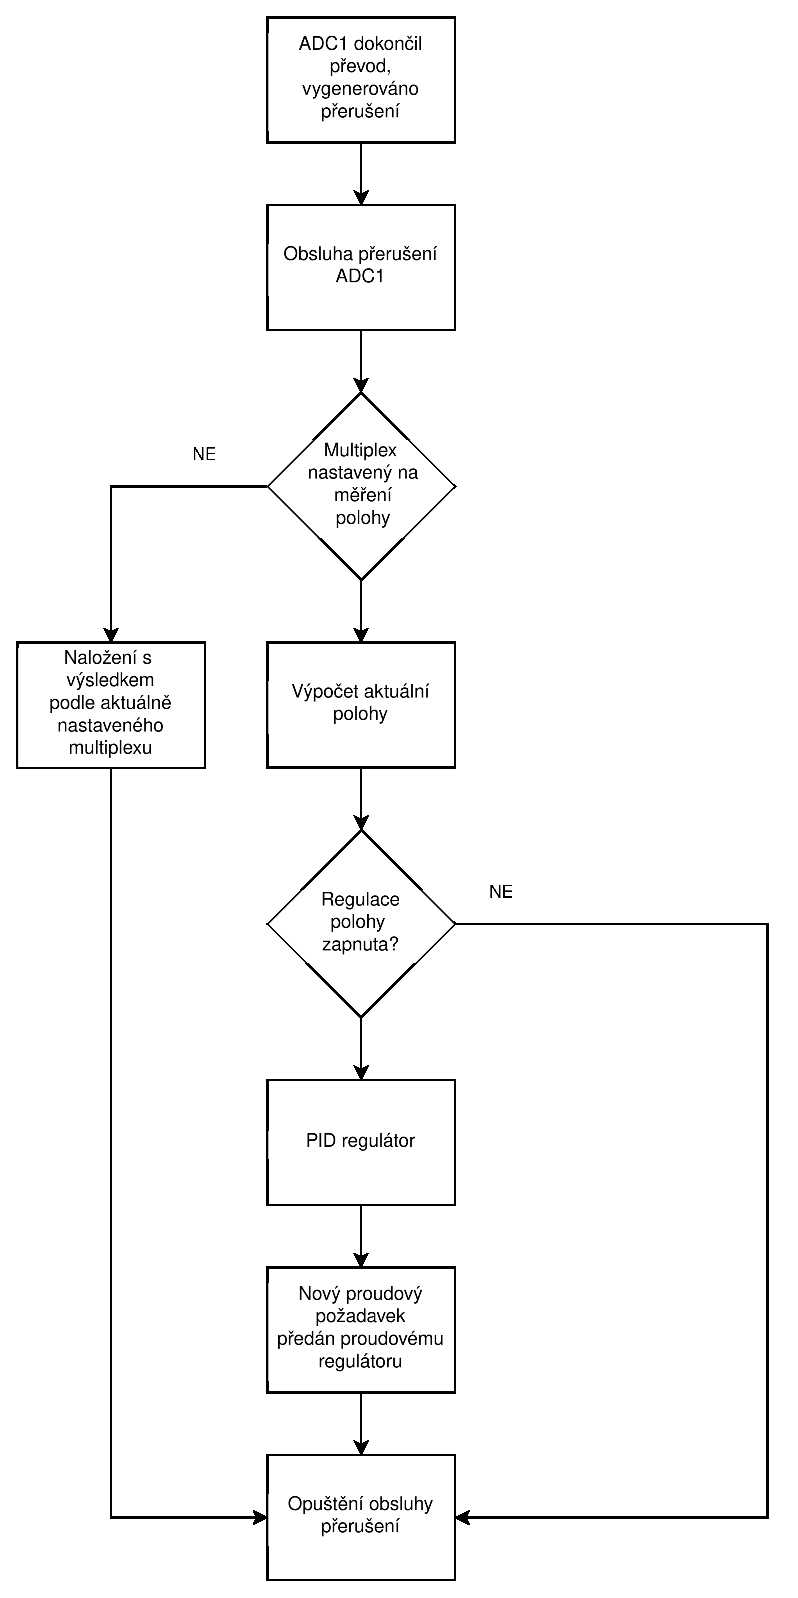
\includegraphics[width=0.6\linewidth]{kapitola4/figures/flowchart_regulator_position.eps}
	\caption{Vývojový diagram regulace polohy}
	\label{fig::flowchart_regulator_position}
\end{figure}

Vývojový diagram regulace polohy je ilustorván na \oref{fig::flowchart_regulator_position}.
Po dokončení převodu je vyvoláno přerušení, ve kterém dochází k výpočtu polohy aktuátoru na základě změřeného napětí.
Převod je realizován pomocí předem zdiskretizované převodní funkce uložené v mikrokontroléru,
viz \nameref{section::hall_perm_magnet}.

Tato převodní funkce byla vytvořena experimentálně.
Nejprve bylo změřeno napětí v závislosti na poloze v několika bodech.
Následně byly naměřené hodnoty interpolovány, zdiskretizovány a uloženy do jednoduchého pole,
kde index odpovídá naměřenému napětí a hodnota v poli reprezentuje odpovídající polohu.
Při samotném převodu se změřené napětí převede na index v tomto poli, jako:

\begin{equation}
	index = \left\lfloor \frac{U_{ADC} - (U_{MIN} + U_{OFFSET})}{(U_{MAX} +  U_{OFFSET}) - (U_{MIN} +  U_{OFFSET})} \cdot ROZSAH \right\rfloor
\end{equation}

kde:
\begin{itemize}
	\item $index$ je index do pole sloužícího jako Look-Up Table,
	\item $U_{ADC}$ je hodnota napětí získaná z ADC převodníku,
	\item $U_{MIN}$ je minimální hodnota napětí v LUT,
	\item $U_{OFFSET}$ je hodnota rozdílu napětí zjištěného v autokalibraci, 
	určujcí rozdíl v napěťové ose mezi funkcí v LUT a skutečnou funkcí,
	\item $U_{MAX}$ je maximální hodnota napětí v LUT,
	\item $ROZSAH$ je velikost pole.
\end{itemize}

Vložením indexu do pole \texttt{h\_interp[index]} dostávám informaci o aktuální poloze.
Regulace polohy je realizována pomocí \textit{PID} regulátoru,
který používá rozdíl požadavku polohy z \textit{DDS} a aktuální polohy z \texttt{h\_interp[index]}.
Parametry \textit{PID} regulátoru byly stanoveny experimentálně na základě odezvy lineárního aktuátoru,
který byl použit v experimentálním vibračním podavači.

Při adresaci \textit{LUT} tabulky pomocí použitého indexu získám aktuální polohu jádra a
získaná hodnota je filtrována exponenciálním klouzavým průměrem pro potlačení příliš rychlých odchylek.
Implementace tohoto filtru odstranila chvění jádra a zlepšila stabilitu polohy.

\begin{lstlisting}[language=C++, caption=Adresace LUT a implementace filtru]
        // Filter parameter (alpha) - Adjust this for smoothing (0.0 < alpha < 1.0)
        static float alpha = 0.33f; // Example: Lower alpha for more smoothing
        static float filtered_position_actual = 0.0f; // Initialize the filter state
        float raw_position_actual = LUT[get_LUT_index()];
        // Apply the EMA filter
        filtered_position_actual = alpha * raw_position_actual + (1.0f - alpha) * filtered_position_actual;
\end{lstlisting}


Výstupem regulátoru polohy je požadovaná hodnota proudu,
která je předána regulátoru proudu implementovanému v metodě \texttt{regulator()} ve třídě \texttt{Current\_source}.

\section{Přímá digitální syntéza}
\label{section::dds}
Pro vytvření střídavých průběhů proudu a pro ovládní polohy linearního aktuátoru bylo použito metod přímé digitální syntézy
(\textit{Direct Digital Synthesis}, \textit{DDS}). 
Tato metoda využívá numerického řízení k vytváření periodických signálů s přesně definovanou frekvencí a fází.

Základem \textit{DDS} je fázový akumulátor a fázový přírůstek:
\begin{itemize}
	\item \textbf{Fázový akumulátor (phase\_accum)}: Jedná se o proměnnou, která uchovává aktuální fázový stav generovaného signálu.
	      S každým vzorkem se jeho hodnota zvyšuje o fázový přírůstek.
	\item \textbf{Fázový přírůstek (phase\_inc)}: Tento parametr určuje krok, o který se fázový akumulátor při každém vzorku posune.
	      Hodnota fázového přírůstku je dána vztahem:
\end{itemize}

\begin{equation}
	f_{OUT} = \frac{\Delta \varphi}{N} \cdot f_{CLK}
	\label{eq::dds}
\end{equation}

kde:
\begin{itemize}
	\item $\Delta \varphi$ je fázový přírůstek,
	\item $f_{OUT}$ je požadovaná výstupní frekvence,
	\item $f_{CLK}$ je hodinová frekvence systému,
	\item $N$ je velikost pole fázového akumulátoru.
\end{itemize}

Maximální frekvence, kterou dokážeme pomoci \textit{DDS} vygenerovat je podle vzorkovacího teorému dána vztahem:
\begin{equation}
	f_{max\_out} = f_{CLK} \cdot \frac{N}{\Delta \varphi_{MAX}} = \frac{f_{CLK}}{2},
	\label{eq::dds_max}
\end{equation}

\subsection{Generování signálu pomocí \textit{DDS}}
Po inkrementaci fázového akumulátoru se jeho hodnota použije jako \texttt{index} pro tabulku vzorků střídavého průběhu \texttt{ac\_lut}.
Tato tabulka obsahuje předpočítané hodnoty chtěné střídavé funkce pro celý rozsah fáze od $0$ do $2\pi$.
Po přetečení hodnoty fázového akumulátoru dochází k restartování jeho hodnoty na 0,
čímž se zajistí periodičnost generovaného signálu.

Výsledný výstupní signál je dán vztahem:

\begin{equation}
	I_{OUT} = Ampl \cdot ac\_lut[phase\_accum] + DC_{OFFSET}
	\label{eq::Iout_DDS}
\end{equation}

kde:
\begin{itemize}
	\item \textbf{Ampl} je uživatelem zadaná amplituda v ampérách, nebo polohový offset v \SI{}{\milli\meter},
	\item \textbf{ac\_lut[phase\_accum]} ukazuje na index pole s uloženou hodnotou odpovídající aktuální fázi,
	\item \textbf{$DC_{OFFSET}$} je stejnosměrný offset přidaný k signálu,
	      může se jednat o proudový offset v ampérách nebo polohový offset v \SI{}{\milli\meter}
\end{itemize}


\subsection{Řešení \textit{DDS} v \textit{MCU}}
\label{section::dds_implementation}

Obsluha syntézy je taktována generováním přerušení při přetečení běžného čítače \textit{TC0}.
Čítač používá jako taktovací hodiny \texttt{GCLK0} s frekvencí \SI{120}{\mega\hertz}
a perioda čítače na \SI{6000}, což generuje přetečení s frekvencí \SI{24}{\kilo\hertz}.
Pole \texttt{ac\_lut} je 2400 floatů veliké.
Pro splnění vzorkovacího teorému, dle \rref{eq::dds_max}, musí platit:

\begin{equation}
	f_{MAX\_OUT} = \frac{f_{CLK}}{2} = \SI{24}{\kilo\hertz},
	\label{eq::dds_max_val}
\end{equation}

V praxi se však obvykle nepoužívá výstupní frekvence blízko $\frac{1}{2}$ taktovací frekvence, 
protože dva vzorky na periodu vedou k velmi špatné rekonsturkci jakéhokoliv signálu.
Vzorky mohou totiž nabývat pouze dvou opačných hodnot, 
což může být například \SI{1}{} a \SI{-1}{}, ale taky \SI{0}{} a \SI{0}{}
a jakéhokoliv kombinace mezi těmito hodnotami.
Navíc vlivem parazitních driftů a posunů kmitočtů dochází k neustálé změně kombinací těchto dvou vzorků.
To vede výstupní signál, který je zatížen parazitní amplitudovou modulací.


A proto se i pro velmi nenáročné aplikace se dá uvažovat maximální užitečná frekvence přibližně jako:

\begin{equation}
	f_{OUT} = f_{MAX\_OUT} = \frac{f_{CLK}}{4},
	\label{eq::dds_real_max_val}
\end{equation}

ovšem pro zajištění ucházejícího harmonického průběhu se doporučuje nejméně 20 vzorků, což znamená:

\begin{equation}
	f_{OUT} = f_{MAX\_OUT} = \frac{f_{CLK}}{20},
\end{equation}


takže po dosazení hodnot implementované \textit{DDS}:

\begin{equation}
	f_{OUT} = f_{MAX\_OUT} = \frac{24000}{4} = \SI{6000}{\hertz},
\end{equation}

respektive:

\begin{equation}
	f_{OUT} = f_{MAX\_OUT} = \frac{24000}{20} = \SI{1200}{\hertz},
\end{equation}

Současná implementace \textit{DDS} umožňuje generování harmonického, trojůhelníkového a obdélníkového signálu,
s libovolným celočíselným fázovým posuvem a stejnosměrným offsetem.
Pro obdélníkový signál lze navíc nastavit střídu a sklon náběžné/doběžné hrany, viz \nameref{section::comunication_protocol}.
Fázový přírůstek je tedy třeba přepočítat při každém zadání frekvence uživatelem.
Z rovnice \eqref{eq::dds_real_max_val} vyplívá maximální frekvence střídavého proudu,
která splňuje požadavek alespoň čtyřech vzorků na jednu periodu signálu, jako \SI{6}{\kilo\hertz}.

Maximální frekvence, kterou může uživatel zvolit je omezena na \SI{2400}{\kilo\hertz},
takže v jedné periodě bude signál tvořen nejméně 10ti vzorky,
ovšem maximální frekvence, kterou zdroj dokáže skutečně vygenerovat je závislá připojené zátěži,
respektive klesá s velikostí indukčnosti zátěže.

\begin{figure}[htpb]
	\centering
	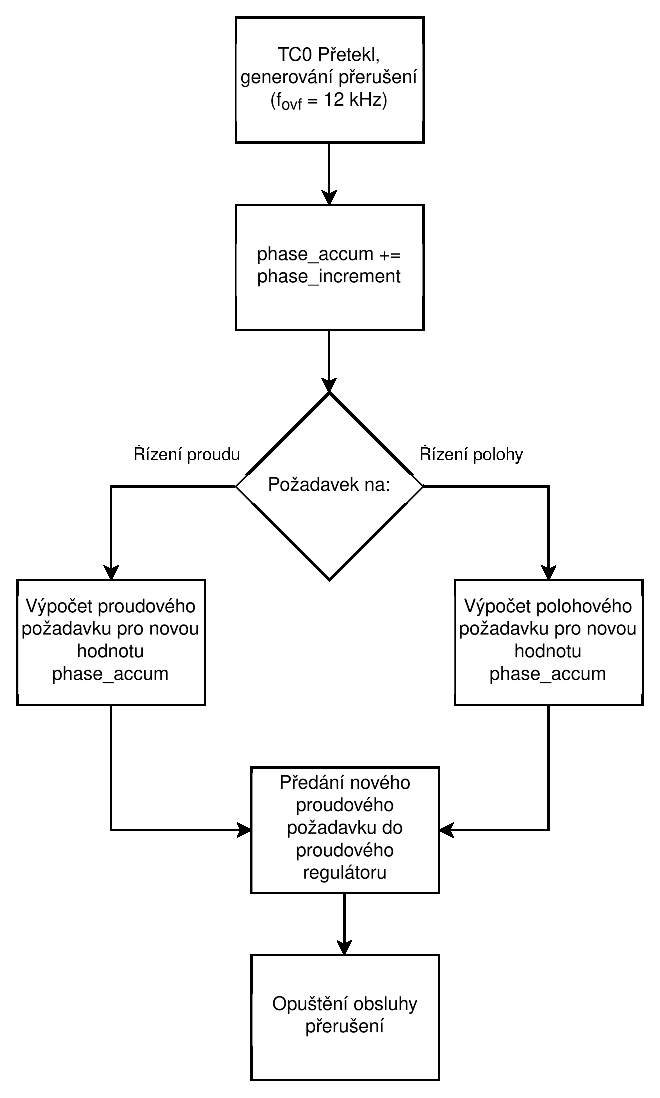
\includegraphics[width=0.5\textwidth]{kapitola4/figures/flowchart_dds.eps} % Cesta k souboru s diagramem
	\caption{Vývojový diagram DDS}
	\label{fig::flowchart_dds}
\end{figure}

V obsluze přerušení dojde k přičtení fázového inkrementu \texttt{phase\_inc} 
k fázovému akumulátoru \texttt{phase\_accum}, viz \ref{fig::flowchart_dds}
a porud vypočítaný dle rovnice \eqref{eq::Iout_DDS}.
Defaultní velikost amplitudy proudu po restartu \texttt{MCU} je \SI{0}{\ampere},
velikost amplitudy polohy \SI{3,5}{\milli\meter}
a OFFSET polohy je \SI{4,5}{\milli\meter}.


\begin{figure}[htpb]
	\centering
	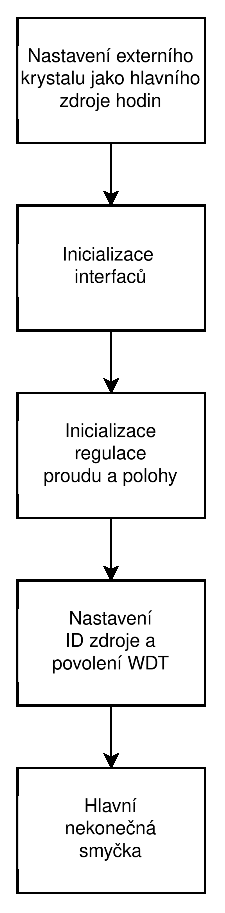
\includegraphics[width=0.15\textwidth]{kapitola4/figures/flowchart_mcu_init.eps} % Cesta k souboru s diagramem
	\caption{Vývojový diagram inicializace}
	\label{fig:mcu_init}
\end{figure}

\section{Běh systému v \texttt{main()}}
\label{section::mcu_main_run}

Po inicializaci systém vstoupí do nekonečné smyčky,
kde se mimo obsluhu přerušení periodicky provádějí následující úkoly:

\begin{enumerate}
	\item Obsluha zdroje proudu pomocí \texttt{aron::Current\_source::handler()}.
	      Tato funkce kontroluje, zda byl odeslán požadavek na vypnutí zdroje.
	      Pokud ano, provede se vypnutí.
	\item Obsluha příjmu zpráv po \textit{UARTu} a \textit{CANu} pomocí \texttt{aron::Communication::rx\_handler()}.
	      Ta zpracovává data přijatá po \textit{UARTu} . Kontroluje FIFO buffer, zda přišla data.
	      Samotný FIFO buffer se plní v přerušení.
	      Také kontroluje, zda přišla nová zpráva po \textit{CAN} sběrnici.
	      Zprávy z \textit{CANu} se do interního bufferu řadiče \texttt{CAN1} ukládají bez činnosti procesoru.
	      Pokud přišla zpráva po kterémkoliv rozhraní, pak ji odešle ke zpracování.
	\item Periodická aktualizace stavových \textit{LED} diod (každých 500 ms).
	\item Periodické spouštění měření teploty (každých 10 s).
	\item Kontrola stisknutí tlačítka. Krátký stisk tlačítka přepíná stav zdroje proudu (zapnuto/vypnuto).
	      Dlouhé podržení tlačítka (déle než 3 sekundy) způsobí restart mikrokontroléru.
	\item Pravidelné krmení Watchdog timeru pomocí funkce \texttt{watch\_dog\_reset()}.
	      Ten se resetuje zápisem hodnoty 0x5A do jeho \texttt{CC} registru.
\end{enumerate}

\begin{figure}[htbp]
	\centering
	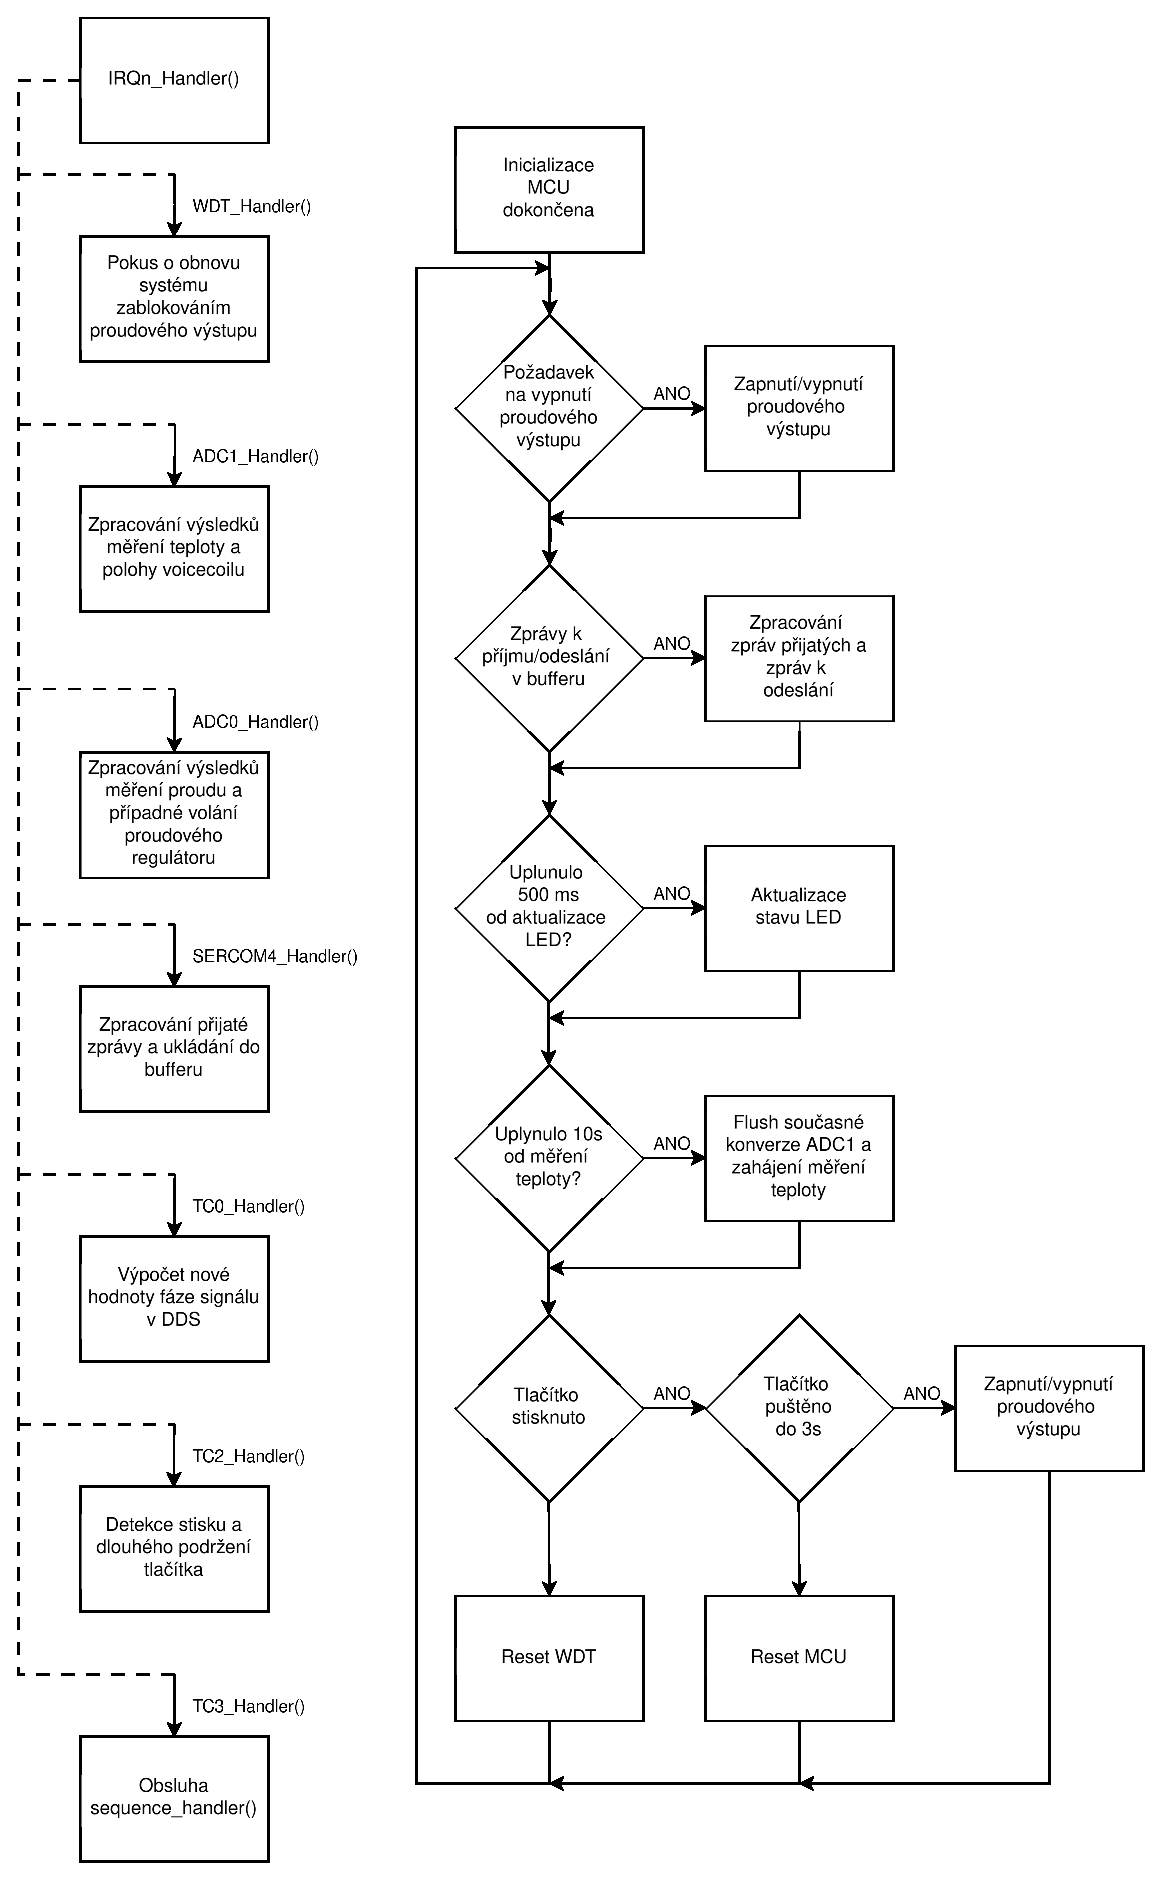
\includegraphics[width=0.9\textwidth]{kapitola4/figures/flowchart_mcu_run.eps} % Cesta k souboru s diagramem
	\caption{Vývojový diagram běhu systému}
	\label{fig:mcu_run}
\end{figure}


\subsection{Popis přerušení}

Systém využívá několik přerušení pro obsluhu různých událostí:

\begin{itemize}
	\item \texttt{WDT\_Handler()}: Obsluha přerušení Watchdog timeru. Vypne výstup v případě, že WDT zahlásí varování.
	      Je to poslední pokus o záchranu běhu systému bez tvrdého restartu.
	\item \texttt{ADC1\_Handler()}: Obsluha přerušení od \texttt{ADC1}.
	      Zpracovává výsledky měření teploty a polohy voicecoilu. Pokud je teplota překročena, zavolá zablokování výstupu.
	      V případě povolené regulace polohy volá regulaci polohy.
	\item \texttt{ADC0\_Handler()}: Obsluha přerušení od \texttt{ADC0}.
	      Zpracovává výsledky měření proudu a případné volání proudového regulátoru
	\item \texttt{SERCOM4\_Handler()}: Obsluha přerušení \texttt{UARTu}.
	      Zpracovává přijaté zprávy a ukládá do bufferu.
	\item \texttt{TC0\_Handler()}: Obsluha přerušení časovače \texttt{TC0}. Používá se pro generování \textit{DDS} signálu.
	\item \texttt{TC2\_Handler()}: Obsluha přerušení časovače \texttt{TC2}. Detekce stisku a dlouhého podržení tlačítka.
	\item \texttt{TC3\_Handler()}: Obsluha přerušení časovače \texttt{TC3}. Obsluha \texttt{sequence\_handler()}.
\end{itemize}